\documentclass[12pt]{article}
\usepackage[utf8]{inputenc}
\usepackage[utf8]{inputenc}
\usepackage{amsmath}
\usepackage{amsthm}
\usepackage{geometry}
\usepackage{amsfonts}
\usepackage{mathrsfs}
\usepackage{bm}
\usepackage{hyperref}
\usepackage[dvipsnames]{xcolor}
\usepackage[inline]{enumitem}
\usepackage{mathtools}
\usepackage{changepage}
\usepackage{lipsum}
\usepackage{tikz}
\usetikzlibrary{matrix, patterns, decorations.pathreplacing, calligraphy}
\usepackage{tikz-cd}
\usepackage[nameinlink]{cleveref}
\geometry{
headheight=15pt,
left=60pt,
right=60pt
}
\setlength{\emergencystretch}{20pt}
\usepackage{fancyhdr}
\pagestyle{fancy}
\fancyhf{}
\lhead{}
\chead{Section 3.3 Exercises}
\rhead{\thepage}
\hypersetup{
    colorlinks=true,
    linkcolor=blue,
    urlcolor=blue
}

\theoremstyle{definition}
\newtheorem*{remark}{Remark}

\newtheoremstyle{exercise}
    {}
    {}
    {}
    {}
    {\bfseries}
    {.}
    { }
    {\thmname{#1}\thmnumber{#2}\thmnote{ (#3)}}
\theoremstyle{exercise}
\newtheorem{exercise}{Exercise 3.3.}

\newtheoremstyle{solution}
    {}
    {}
    {}
    {}
    {\itshape\color{magenta}}
    {.}
    { }
    {\thmname{#1}\thmnote{ #3}}
\theoremstyle{solution}
\newtheorem*{solution}{Solution}

\Crefformat{exercise}{#2Exercise 3.3.#1#3}

\newcommand{\interior}[1]{%
  {\kern0pt#1}^{\mathrm{o}}%
}
\newcommand{\ts}{\textsuperscript}
\newcommand{\setcomp}[1]{#1^{\mathsf{c}}}
\newcommand{\quand}{\quad \text{and} \quad}
\newcommand{\N}{\mathbf{N}}
\newcommand{\Z}{\mathbf{Z}}
\newcommand{\Q}{\mathbf{Q}}
\newcommand{\I}{\mathbf{I}}
\newcommand{\R}{\mathbf{R}}
\newcommand{\C}{\mathbf{C}}

\DeclarePairedDelimiter\abs{\lvert}{\rvert}
% Swap the definition of \abs* and \norm*, so that \abs
% and \norm resizes the size of the brackets, and the 
% starred version does not.
\makeatletter
\let\oldabs\abs
\def\abs{\@ifstar{\oldabs}{\oldabs*}}
%
\let\oldnorm\norm
\def\norm{\@ifstar{\oldnorm}{\oldnorm*}}
\makeatother

\setlist[enumerate,1]{label={(\alph*)}}

\begin{document}

\section{Section 3.3 Exercises}

Exercises with solutions from Section 3.3 of \hyperlink{ua}{[UA]}.

\begin{exercise}
\label{ex:1}
    Show that if \( K \) is compact and non-empty, then \( \sup K \) and \( \inf K \) both exist and are elements of \( K \).
\end{exercise}

\begin{solution}
    By Theorem 3.3.8, \( K \) must be closed and bounded. Then since \( K \) is non-empty and bounded, \( \sup K \) and \( \inf K \) both exist. For each \( n \in \N \), we can find elements \( x_n \) and \( y_n \) in \( K \) satisfying
    \[
        \sup K - \frac{1}{n} < x_n \leq \sup K \quand \inf K \leq y_n < \inf K + \frac{1}{n}.
    \]
    It follows that \( \lim x_n = \sup K \) and \( \lim y_n = \inf K \), so that \( \sup K \) and \( \inf K \) are limit points of \( K \). Since \( K \) is closed, \( \sup K \) and \( \inf K \) must belong to \( K \).
\end{solution}

\begin{exercise}
\label{ex:2}
    Decide which of the following sets are compact. For those that are not compact, show how Definition 3.3.1 breaks down. In other words, give an example of a sequence contained in the given set that does not possess a subsequence converging to a limit in the set.
    \begin{enumerate}
        \item \( \N \).

        \item \( \Q \cap [0, 1] \).

        \item The Cantor set.

        \item \( \{ 1 + 1/2^2 + 1/3^2 + \cdots + 1/n^2 : n \in \N \} \).

        \item \( \{ 1, 1/2, 2/3, 3/4, 4/5, \ldots \} \).
    \end{enumerate}
\end{exercise}

\begin{solution}
    \begin{enumerate}
        \item \( \N \) is not compact. Consider the sequence \( (n) \), which is increasing and unbounded. As shown in the solution to \href{https://lew98.github.io/Mathematics/UA_Section_2_7_Exercises.pdf}{Exercise 2.7.6 (c)}, such sequences do not have convergent subsequences.

        \item \( \Q \cap [0, 1] \) is not compact. Let \( x = \tfrac{\sqrt{2}}{2} \in (0, 1) \). By Theorem 3.2.10, there is a sequence of rational numbers \( (x_n) \) converging to \( x \). Since \( 0 < x < 1 \), this sequence must eventually be contained in \( (0, 1) \). By removing a finite number of terms from the sequence if necessary, which will not affect convergence, we may assume that the sequence is entirely contained in \( \Q \cap [0, 1] \). Then by Theorem 2.5.2, every subsequence of \( (x_n) \) also converges to \( x \), which does not belong to \( \Q \cap [0, 1] \).

        \item The Cantor set is compact, since it is closed and bounded.

        \item Let \( E \) be the set in question and let \( s_n = \sum_{j=1}^n \tfrac{1}{j^2} \). Then \( (s_n) \) is contained in \( E \) and from Chapter 2 we know that \( \lim s_n = L \) for some \( L \in \R \). As shown in \href{https://lew98.github.io/Mathematics/UA_Section_3_2_Exercises.pdf}{Exercise 3.2.3 (d)}, \( L \) does not belong to \( E \). Since all subsequences of \( s_n \) also converge to \( L \), we see that \( E \) is not compact.

        \item Let \( E \) be the set in question, i.e.\
        \[
            E = \{ 1 \} \cup \left\{ 1 - \tfrac{1}{n} : n \in \N \right\}.
        \]
        Using a similar argument to the one given in \href{https://lew98.github.io/Mathematics/UA_Section_3_2_Exercises.pdf}{Exercise 3.2.2}, we see that 1 is the only limit point of \( E \). It follows that \( E \) is closed and bounded, and hence compact.
    \end{enumerate}
\end{solution}

\begin{exercise}
\label{ex:3}
    Prove the converse of Theorem 3.3.4 by showing that if a set \( K \subseteq \R \) is closed and bounded, then it is compact.
\end{exercise}

\begin{solution}
    Suppose that \( K \subseteq \R \) is closed and bounded and let \( (x_n) \) be an arbitrary sequence contained in \( K \). Then \( (x_n) \) is a bounded sequence, so the Bolzano-Weierstrass Theorem implies that there exists a subsequence \( (x_{n_k}) \) such that \( \lim_k x_{n_k} = x \) for some \( x \in \R \). Since \( (x_{n_k}) \) is contained in \( K \), we see that \( x \) must be a limit point of \( K \), and since \( K \) is closed, we then have \( x \in K \). It follows that any sequence contained in \( K \) has a subsequence which converges to some element of \( K \), i.e.\ \( K \) is compact.
\end{solution}

\begin{exercise}
\label{ex:4}
    Assume \( K \) is compact and \( F \) is closed. Decide if the following sets are definitely compact, definitely closed, both, or neither.
    \begin{enumerate}
        \item \( K \cap F \)

        \item \( \overline{\setcomp{F} \cup \setcomp{K}} \)

        \item \( K \setminus F = \{ x \in K : x \not\in F \} \)

        \item \( \overline{K \cap \setcomp{F}} \)
    \end{enumerate}
\end{exercise}

\begin{solution}
    \begin{enumerate}
        \item \( K \) is closed since it is compact, so \( K \cap F \) is the intersection of two closed sets and hence is definitely closed. It is easy to see that the intersection of a bounded set with any other set is again bounded, so since \( K \) is bounded by virtue of being compact, we see that \( K \cap F \) is bounded as well as closed. It follows that \( K \cap F \) is definitely compact.

        \item The closure of any set is closed, so \( \overline{\setcomp{F} \cup \setcomp{K}} \) is definitely closed. However, \( \overline{\setcomp{F} \cup \setcomp{K}} \) cannot be compact since it is unbounded. To see this, let us first show that if \( E \subseteq \R \) is bounded, then \( \setcomp{E} \) is unbounded. Since \( E \) is bounded, there exists an \( M > 0 \) such that \( E \subseteq [-M, M] \). It follows that \( ((-\infty, M) \cup (M, \infty)) \subseteq \setcomp{E} \), whence \( \setcomp{E} \) is unbounded. Returning to the set \( \overline{\setcomp{F} \cup \setcomp{K}} \), we have that \( K \) is bounded since it is compact and thus \( \setcomp{K} \) is unbounded. Then since
        \[
            \setcomp{K} \subseteq \setcomp{F} \cup \setcomp{K} \subseteq \overline{\setcomp{F} \cup \setcomp{K}},
        \]
        we see that \( \overline{\setcomp{F} \cup \setcomp{K}} \) must also be unbounded. It follows that \( \overline{\setcomp{F} \cup \setcomp{K}} \) cannot be compact.

        \item Since \( K \) is bounded, \( K \setminus F \) must also be bounded, and hence \( K \setminus F \) is compact if and only if it is closed. \( K \setminus F \) could be compact/closed: for example, taking \( F = \emptyset \). \( K \setminus F \) could also fail to be compact/closed. For example, if we take \( K = [-2, 2] \) and \( F = [-1, 1] \), then \( K \setminus F = [-2, 1) \cup (1, 2] \), which is not compact/closed.

        \item First, let us show that if \( E \subseteq \R \) is bounded by some \( M > 0 \), then so is \( \overline{E} \). Suppose that \( x \in \R \) is a limit point of \( E \). Then there is a sequence \( (x_n) \) contained in \( E \) such that \( \lim x_n = x \). Since \( -M \leq x_n \leq M \) for all \( n \in \N \), the Order Limit Theorem implies that \( -M \leq x \leq M \) and hence we see that \( \overline{E} \) is also bounded by \( M \).

        Returning to the question, note that since \( K \) is bounded, \( K \cap \setcomp{F} \) must also be bounded. Then by the previous paragraph, \( \overline{K \cap \setcomp{F}} \) is bounded. Thus \( \overline{K \cap \setcomp{F}} \) is compact since it is closed and bounded.
    \end{enumerate}
\end{solution}

\begin{exercise}
\label{ex:5}
    Decide whether the following propositions are true or false. If the claim is valid, supply a short proof, and if the claim is false, provide a counterexample.
    \begin{enumerate}
        \item The arbitrary intersection of compact sets is compact.

        \item The arbitrary union of compact sets is compact.

        \item Let \( A \) be arbitrary, and let \( K \) be compact. Then, the intersection \( A \cap K \) is compact.

        \item If \( F_1 \supseteq F_2 \supseteq F_3 \supseteq F_4 \supseteq \cdots \) is a nested sequence of nonempty closed sets, then the intersection \( \bigcap_{n=1}^{\infty} F_n \neq \emptyset \).
    \end{enumerate}
\end{exercise}

\begin{solution}
    \begin{enumerate}
        \item This is true. Suppose we have some collection \( \{ K_a : a \in A \} \) of compact sets. Then each \( K_a \) must be closed and bounded and so the intersection \( K := \bigcap_{a \in A} K_a \) is also closed and bounded. Thus \( K \) is compact.

        \item This is false. For each \( n \in \N \), let \( K_n = [0, n] \). Then each \( K_n \) is closed and bounded and hence compact. However, \( \bigcup_{n=1}^{\infty} K_n = [0, \infty) \), which is unbounded and hence not compact.

        \item This is false. Let \( A = (0, 1) \) and \( K = [0, 1] \). Then \( K \) is compact since it is closed and bounded, but \( A \cap K = (0, 1) \), which is not closed and hence not compact.

        \item This is false. For each \( n \in \N \), let \( F_n = [n, \infty) \). Then each \( F_n \) is non-empty and closed, and the sequence \( (F_n) \) is nested. However, \( \bigcap_{n=1}^{\infty} F_n = \emptyset \).
    \end{enumerate}
\end{solution}

\begin{exercise}
\label{ex:6}
    This exercise is meant to illustrate the point made in the opening paragraph to Section 3.3. Verify that the following three statements are true if every blank is filled in with the word ``finite.'' Which are true if every blank is filled in with the word ``compact''? Which are true if every blank is filled in with the word ``closed''?
    \begin{enumerate}
        \item Every \rule{1cm}{0.15mm} set has a maximum.

        \item If \( A \) and \( B \) are \rule{1cm}{0.15mm}, then \( A + B = \{ a + b : a \in A, b \in B \} \) is also \rule{1cm}{0.15mm}.

        \item If \( \{ A_n : n \in \N \} \) is a collection of \rule{1cm}{0.15mm} sets with the property that every finite subcollection has a nonempty intersection, then \( \bigcap_{n=1}^{\infty} A_n \) is nonempty as well.
    \end{enumerate}
\end{exercise}

\begin{solution}
    \begin{enumerate}
        \item Let us show that every non-empty finite set has a maximum, by induction on the number of elements in the set. If \( E \subseteq \R \) has a single element \( x \), then clearly \( x \) is the maximum of \( E \). Suppose that any subset of \( \R \) with \( n \) elements has a maximum and suppose that \( E \subseteq \R \) has \( n + 1 \) elements. Pick any \( x \in E \) and consider the set \( E \setminus \{ x \} \), which has \( n \) elements. Then by assumption, this set has a maximum element \( y \). There are now two cases. If \( x \leq y \), then \( y \) is the maximum of \( E \), and if \( x > y \), then \( x \) is the maximum of \( E \). In either case, \( E \) has a maximum element. It follows by induction that any non-empty finite set has a maximum.

        It is true that any non-empty compact set has a maximum, as we showed in \Cref{ex:1}. However, not every closed set has a maximum. For example, \( \R \) is closed but has no maximum element.

        \item If \( A \) is finite with \( m \) elements and \( B \) is finite with \( n \) elements, then \( A + B \) can have at most \( mn \) elements and hence is also finite.

        Suppose that \( A \) and \( B \) are compact and let \( (x_n) \) be a sequence contained in \( A + B \). Then there must be sequences \( (a_n) \) contained in \( A \) and \( (b_n) \) contained in \( B \) such that \( x_n = a_n + b_n \) for each \( n \in \N \). Since \( A \) is compact, the sequence \( (a_n) \) has a subsequence \( (a_{n_k}) \) such that \( \lim_k a_{n_k} = a \) for some \( a \in A \). Since \( B \) is compact, the sequence \( (b_{n_k}) \) has a subsequence \( (b_{n_{k_l}}) \) such that \( \lim_l b_{n_{k_l}} = b \) for some \( b \in B \). Then observe that
        \[
            \lim_l x_{n_{k_l}} = \lim_l \left( a_{n_{k_l}} + b_{n_{k_l}} \right) = \lim_l a_{n_{k_l}} + \lim_l b_{n_{k_l}} = a + b \in A + B.
        \]
        It follows that \( A + B \) is compact.

        It is not necessarily the case that \( A + B \) is closed for closed sets \( A \) and \( B \). For a counterexample, let \( A = \N \) and let \( B = \left\{ -n + \tfrac{1}{n} : n \in \N \right\} \). Then for each \( n \in \N \), we have \( n + \left( -n + \tfrac{1}{n} \right) = \tfrac{1}{n} \in A + B \). It follows that 0 is a limit point of \( A + B \). However, any element of \( A + B \) is of the form \( k + \tfrac{1}{n} \) for some \( k \in \Z \) and \( n \in \N \). Since 0 is certainly not of this form, we see that \( A + B \) fails to contain the limit point 0. Thus \( A + B \) is not closed.

        \item Suppose \( \{ A_n : n \in \N \} \) is a collection of finite sets with the property that every finite subcollection has a non-empty intersection. For each \( k \in \N \), let \( m_k \) be the number of elements in \( \bigcap_{n=1}^k A_n \). By assumption, \( m_k \geq 1 \) for all \( k \in \N \). It is also clear that
        \[
            m_1 \geq m_2 \geq m_3 \geq \cdots \geq m_k \geq \cdots.
        \]
        This sequence must eventually be constant; it could decrease at most \( m_1 - 1 \) times. So there exists a positive integer \( K \) such that
        \[
            k \geq K \implies m_k = m_K \iff \bigcap_{n=1}^k A_n = \bigcap_{n=1}^K A_n.
        \]
        Since \( m_K \geq 1 \), there exists some \( x \in \bigcap_{n=1}^K A_n \). Then since \( x \in \bigcap_{n=1}^k A_n \) for all \( k \geq K \), we have \( x \in \bigcap_{n=1}^{\infty} A_n \).

        Suppose \( \{ A_n : n \in \N \} \) is a collection of compact sets with the property that every finite subcollection has a non-empty intersection. For \( m \in \N \), define \( K_m = \bigcap_{n=1}^m A_n \). Then each \( K_m \) is non-empty by assumption, each \( K_m \) is compact by \Cref{ex:5} (a), we have \( \bigcap_{m=1}^{\infty} K_m = \bigcap_{n=1}^{\infty} A_n \), and the sequence \( (K_m) \) satisfies
        \[
            K_1 \supseteq K_2 \supseteq K_3 \supseteq \cdots \supseteq K_m \supseteq \cdots.
        \]
        Then by Theorem 3.3.5, the intersection \( \bigcap_{m=1}^{\infty} K_m = \bigcap_{n=1}^{\infty} A_n \) is non-empty.

        For each \( n \in \N \), let \( A_n \) be the closed set \( [n, \infty) \). For a finite subcollection \( \{ A_{n_1}, \ldots, A_{n_m} \} \), we have
        \[
            \bigcap_{i=1}^m A_{n_i} = [N, \infty) \neq \emptyset,
        \]
        where \( N = \max_{1 \leq i \leq m} n_i \). However, \( \bigcap_{n=1}^{\infty} A_n = \emptyset \).
    \end{enumerate}
\end{solution}

\begin{exercise}
\label{ex:7}
    As some more evidence of the surprising nature of the Cantor set, follow these steps to show that the sum \( C + C = \{ x + y : x, y \in C \} \) is equal to the closed interval \( [0, 2] \). (Keep in mind that \( C \) has zero length and contains no intervals.)

    Because \( C \subseteq [0, 1], C + C \subseteq [0, 2], \) so we only need to prove the reverse inclusion \( [0, 2] \subseteq \{ x + y : x, y \in C \} \). Thus, given \( s \in [0, 2] \), we must find two elements \( x, y \in C \) satisfying \( x + y = s \).
    \begin{enumerate}
        \item Show that there exist \( x_1, y_1 \in C_1 \) for which \( x_1 + y_1 = s \). Show in general that, for an arbitrary \( n \in \N \), we can always find \( x_n, y_n \in C_n \) for which \( x_n + y_n = s \).

        \item Keeping in mind that the sequences \( (x_n) \) and \( (y_n) \) do not necessarily converge, show how they can nevertheless be used to produce the desired \( x \) and \( y \) in \( C \) satisfying \( x + y = s \).
    \end{enumerate}
\end{exercise}

\begin{solution}
    \begin{enumerate}
        \item If \( \tfrac{s}{2} \in C_1 = \left[ 0, \tfrac{1}{3} \right] \cup \left[ \tfrac{2}{3}, 1 \right] \), then take \( x_1 = y_1 = \tfrac{s}{2} \), and if \( \tfrac{s}{2} \in \left( \tfrac{1}{3}, \tfrac{2}{3} \right) \), then take \( x_1 = \tfrac{s}{2} - \tfrac{1}{3} \) and \( y_1 = \tfrac{s}{2} + \tfrac{1}{3} \). In either case, we have \( x_1, y_1 \in C_1 \) and \( x_1 + y_1 = s \). Geometrically, we have shown that for any \( s \in [0, 2] \), the line given by \( x + y = s \) must intersect the set \( C_1 \times C_1 \subseteq \R^2 \); see \Cref{fig:1}, which shows the set \( C_1 \times C_1 \) as well as the lines \( x + y = s \) for several values of \( s \).

        \begin{figure}[h]
            \centering
            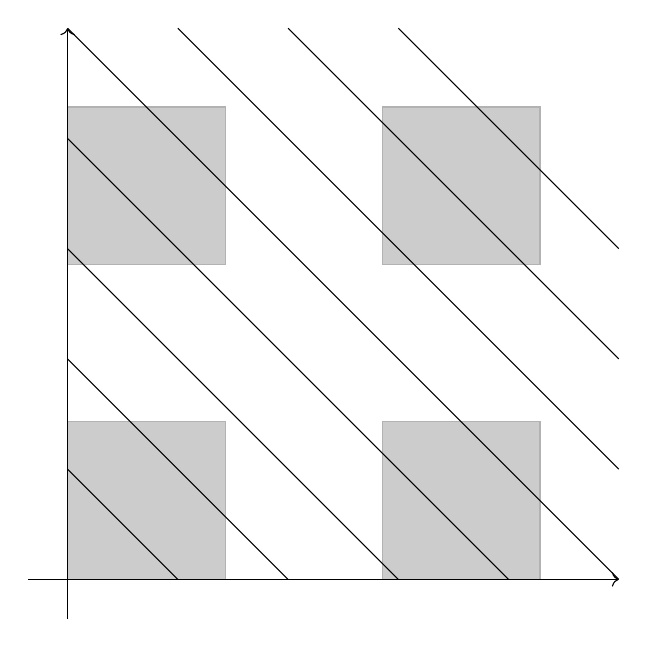
\begin{tikzpicture}
                % C_1 x C_1
                \filldraw[fill=gray!40, draw=gray!60]
                    (0, 0) rectangle (2, 2)
                    (4, 0) rectangle (6, 2)
                    (0, 4) rectangle (2, 6)
                    (4, 4) rectangle (6, 6);

                % x + y = s
                \draw
                    (4.2, 7) -- (7, 4.2)
                    (2.8, 7) -- (7, 2.8)
                    (1.4, 7) -- (7, 1.4)
                    (0, 7) -- (7, 0)
                    (0, 5.6) -- (5.6, 0)
                    (0, 4.2) -- (4.2, 0)
                    (0, 2.8) -- (2.8, 0)
                    (0, 1.4) -- (1.4, 0);
                
                % Axes
                \draw[->] (-0.5, 0) -- (7, 0);
                \draw[->] (0, -0.5) -- (0, 7);
            \end{tikzpicture}
            \caption{\( C_1 \times C_1 \)} \label{fig:1}
        \end{figure}

        Let us argue inductively that for any \( n \in \N \), we can find \( x_n, y_n \in C_n \) such that \( x_n + y_n = s \). The base case \( n = 1 \) was handled above, so suppose that for some \( n \in \N \) we have \( x_n, y_n \in C_n \) such that \( x_n + y_n = s \). Since \( C_n \) consists of \( 2^n \) closed intervals each of length \( 3^{-n} \), the set \( C_n \times C_n \) consists of \( (2^n)^2 \) closed squares each with side length \( 3^{-n} \). Geometrically, the induction hypothesis guarantees that the line \( x + y = s \) intersects the set \( C_n \times C_n \) and thus must intersect one of the \( (2^n)^2 \) closed squares. Moving from \( C_n \) to \( C_{n+1} \), the middle third of each of the \( 2^n \) intervals is removed. This has the effect of splitting each of the \( (2^n)^2 \) squares of \( C_n \times C_n \) into four subsquares; see \Cref{fig:2}. \( C_{n+1} \times C_{n+1} \) then consists of the collection of these subsquares.
        
        Now we make the observation that this situation is essentially the same as in the base case; given that the line \( x + y = s \) intersects one of the squares of \( C_n \times C_n \), it must intersect at least one of the four subsquares after we remove the middle third of the sides of the square; see \Cref{fig:2} again. We are then guaranteed the existence of some \( x_{n+1}, y_{n+1} \in C_{n+1} \) such that \( x_{n+1} + y_{n+1} = s \). This completes the induction step.

        \begin{figure}[h]
            \centering
            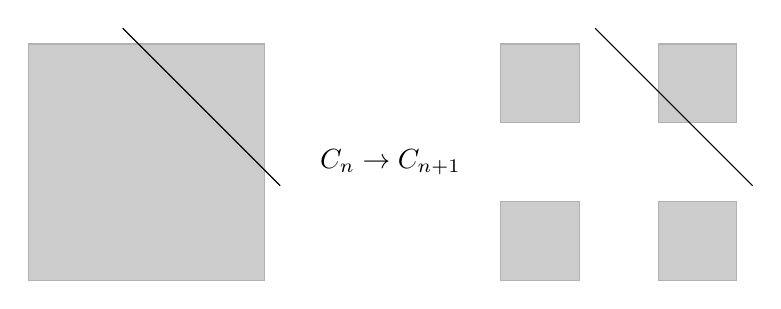
\begin{tikzpicture}
                \filldraw[fill=gray!40, draw=gray!60]
                    (0, 0) rectangle (3, 3)
                    (6, 0) rectangle (7, 1)
                    (6, 2) rectangle (7, 3)
                    (8, 0) rectangle (9, 1)
                    (8, 2) rectangle (9, 3);

                \path (4.6, 1.5) node {\( C_n \to C_{n+1} \)};

                \draw
                    (1.2, 3.2) -- (3.2, 1.2)
                    (7.2, 3.2) -- (9.2, 1.2);
            \end{tikzpicture}
            \caption{Subsquares of \( C_n \times C_n \) and \( C_{n+1} \times C_{n+1} \)} \label{fig:2}
        \end{figure}

        \item The sequence \( (x_n) \) is certainly bounded, so by the Bolzano-Weierstrass Theorem it has a convergent subsequence \( (x_{n_k}) \to x \) for some \( x \in \R \). Similarly, the sequence \( (y_{n_k}) \) is bounded and hence has a convergent subsequence \( (y_{n_{k_l}}) \to y \) for some \( y \in \R \). Since the sequence \( (C_n) \) is nested, we have \( x_{n_{k_l}} \in C_1 \) for all \( l \in \N \). Then since \( C_1 \) is closed, it must be the case that \( x \in C_1 \). The terms \( x_{n_{k_l}} \) belong to \( C_2 \) provided \( n_{k_l} \geq 2 \), i.e.\ all but a finite number of terms of \( (x_{n_{k_l}}) \) belong to \( C_2 \). Since \( C_2 \) is closed, it must be the case that \( x \in C_2 \). Continuing in this fashion, we see that \( x \in C_n \) for all \( n \in \N \), i.e.\ \( x \in C \). Similarly, we obtain \( y \in C \). Now observe that on one hand,
        \[
            \lim_l \left( x_{n_{k_l}} + y_{n_{k_l}} \right) = x + y.
        \]
        On the other hand,
        \[
            \lim_l \left( x_{n_{k_l}} + y_{n_{k_l}} \right) = \lim_l s = s.
        \]
        Since limits are unique, we may conclude that \( x + y = s \).
    \end{enumerate}
\end{solution}

\begin{exercise}
\label{ex:8}
    Let \( K \) and \( L \) be nonempty compact sets, and define
    \[
        d = \inf \{ \abs{x - y} : x \in K \text{ and } y \in L \}.
    \]
    This turns out to be a reasonable definition for the \textit{distance} between \( K \) and \( L \).
    \begin{enumerate}
        \item If \( K \) and \( L \) are disjoint, show \( d > 0 \) and that \( d = \abs{x_0 - y_0} \) for some \( x_0 \in K \) and \( y_0 \in L \).

        \item Show that it's possible to have \( d = 0 \) if we assume only that the disjoint sets \( K \) and \( L \) are closed.
    \end{enumerate}
\end{exercise}

\begin{solution}
    \begin{enumerate}
        \item Let \( E = \{ \abs{x - y} : x \in K \text{ and } y \in L \} \). Then \( E \) is non-empty since \( K \) and \( L \) are non-empty and \( E \) is clearly bounded below by 0. Thus \( d = \inf E \) exists. For each \( n \in \N \), there exist elements \( x_n \in K \) and \( y_n \in L \) such that
        \[
            d \leq \abs{x_n - y_n} < d + \tfrac{1}{n}.
        \]
        It follows that \( \lim_n \abs{x_n - y_n} = d \). Since \( (x_n) \) is entirely contained in the compact set \( K \), we are guaranteed the existence of a convergent subsequence \( (x_{n_k}) \to x_0 \) for some \( x_0 \in K \). Similarly, since the sequence \( (y_{n_k}) \) is entirely contained in the compact set \( L \), we are guaranteed the existence of a convergent subsequence \( (y_{n_{k_l}}) \to y_0 \) for some \( y_0 \in L \). Then we have
        \[
            \lim_l \abs{x_{n_{k_l}} - y_{n_{k_l}}} = \abs{x_0 - y_0}.
        \]
        However, we must also have \( \lim_l \abs{x_{n_{k_l}} - y_{n_{k_l}}} = d \). It follows that \( \abs{x_0 - y_0} = d \). Since \( K \) and \( L \) are disjoint, it must be the case that \( x_0 \neq y_0 \) and hence that \( d > 0 \).

        \item Let \( K = \N \) and \( L = \{ n + n^{-1} : n \in \N \} \). Then \( K \) and \( L \) are non-empty and disjoint. Furthermore, since
        \[
            \setcomp{K} = (-\infty, 1) \cup \bigcup_{n=1}^{\infty} (n, n + 1) \quand \setcomp{L} = (-\infty, 2) \cup \bigcup_{n=1}^{\infty} (n + n^{-1}, n + 1 + (n + 1)^{-1}),
        \]
        we see that \( \setcomp{K} \) and \( \setcomp{L} \) are both open and hence that \( K \) and \( L \) are both closed. Letting \( E = \{ \abs{x - y} : x \in K \text{ and } y \in L \} \) again, note that for each \( n \in \N \), by taking \( n \in K \) and \( n + n^{-1} \in L \), we have \( n^{-1} \in E \). It follows that \( d = \inf E = 0 \).
    \end{enumerate}
\end{solution}

\begin{exercise}
\label{ex:9}
    Follow these steps to prove the final implication in Theorem 3.3.8.

    Assume \( K \) satisfies (i) and (ii), and let \( \{ O_{\lambda} : \lambda \in \Lambda \} \) be an open cover for \( K \). For contradiction, let's assume that no finite subcover exists. Let \( I_0 \) be a closed interval containing \( K \).
    \begin{enumerate}
        \item Show that there exists a nested sequence of closed intervals \( I_0 \supseteq I_1 \supseteq I_2 \supseteq \cdots \) with the property that, for each \( n \), \( I_n \cap K \) cannot be finitely covered and \( \lim \abs{I_n} = 0 \).

        \item Argue that there exists an \( x \in K \) such that \( x \in I_n \) for all \( n \).

        \item Because \( x \in K \), there must exist an open set \( O_{\lambda_0} \) from the original collection that contains \( x \) as an element. Explain how this leads to the desired contradiction.
    \end{enumerate}
\end{exercise}

\begin{solution}
    \begin{enumerate}
        \item Let us proceed by induction. For the base case, \( I_0 \cap K = K \) cannot be covered by any finite subcollection of \( \{ O_{\lambda} : \lambda \in \Lambda \} \) and we have \( \abs{I_0} = 2^0 \abs{I_0} \).
        
        Suppose that after \( n \) steps we have chosen nested closed intervals \( I_0 \supseteq I_1 \supseteq I_2 \supseteq \cdots \supseteq I_{n-1} \) such that, for each \( 0 \leq m \leq n - 1 \), \( I_m \cap K \) cannot be covered by any finite subcollection of \( \{ O_{\lambda} : \lambda \in \Lambda \} \) and \( \abs{I_m} = 2^{-m} \abs{I_0} \). Suppose that \( I_{n-1} = [a, c] \) and let \( b = \tfrac{a + c}{2} \). Note that if both of the sets \( [a, b] \cap K \) and \( [b, c] \cap K \) could be covered by a finite subcollection of \( \{ O_{\lambda} : \lambda \in \Lambda \} \), then \( I_{n-1} \) could also be finitely covered. By assumption, this is not the case, so at least of the one intervals \( [a, b] \) or \( [b, c] \) must have the property that its intersection with \( K \) cannot be finitely covered. Let \( I_n \) be this interval and note that \( I_n \subseteq I_{n-1} \). Furthermore, since \( \abs{I_{n-1}} = 2^{-n + 1} \abs{I_0} \), we have \( \abs{I_n} = 2^{-n} \abs{I_0} \). This completes the induction step and hence we obtain the desired sequence of nested closed intervals.

        \item For each \( n \in \N, I_n \cap K \) is the intersection of two compact sets and hence is itself compact. Furthermore, since the sequence \( (I_n) \) is nested, the sequence \( (I_n \cap K) \) is also nested. Then by Theorem 3.3.5, there exists some \( x \in \bigcap_{n=1}^{\infty} (I_n \cap K) = K \cap \bigcap_{n=1}^{\infty} I_n \).

        \item Since \( x \) belongs to the open set \( O_{\lambda_0} \), there exists an \( \epsilon > 0 \) such that \( V_{\epsilon}(x) \subseteq O_{\lambda_0} \). Since \( \lim \abs{I_n} = 0 \), there exists an \( N \in \N \) such that \( \abs{I_n} < \tfrac{\epsilon}{2} \) for \( n \geq N \). Then since \( x \in I_N \), we must have \( I_N \subseteq V_{\epsilon}(x) \) and hence \( I_N \cap K \subseteq V_{\epsilon}(x) \). This implies that \( I_N \cap K \subseteq O_{\lambda_0} \), contradicting the fact that \( I_N \cap K \) cannot be covered by any finite subcollection of \( \{ O_{\lambda} : \lambda \in \Lambda \} \).
    \end{enumerate}
\end{solution}

\begin{exercise}
\label{ex:10}
    Here is an alternate proof to the one given in \Cref{ex:9} for the final implication in the Heine-Borel Theorem.

    Consider the special case where \( K \) is a closed interval. Let \( \{ O_{\lambda} : \lambda \in \Lambda \} \) be an open cover for \( [a, b] \) and define \( S \) to be the set of all \( x \in [a, b] \) such that \( [a, x] \) has a finite subcover from \( \{ O_{\lambda} : \lambda \in \Lambda \} \).
    \begin{enumerate}
        \item Argue that \( S \) is nonempty and bounded, and thus \( s = \sup S \) exists.

        \item Now show \( s = b \), which implies \( [a, b] \) has a finite subcover.

        \item Finally, prove the theorem for an arbitrary closed and bounded set \( K \).
    \end{enumerate}
\end{exercise}

\begin{solution}
    \begin{enumerate}
        \item Since \( a \in [a, b] \), there must be some \( O_{\lambda_0} \) such that \( a \in O_{\lambda_0} \). Hence \( [a, a] \) is finitely covered and so \( a \in S \). Evidently, \( S \) is bounded above by \( b \). Thus by completeness, \( s = \sup S \) exists.

        \item Seeking a contradiction, suppose that \( s < b \), so that \( \epsilon_1 := \tfrac{b - s}{2} > 0 \). Since \( s \in [a, b] \), there exists some \( O_{\lambda_0} \) such that \( s \in O_{\lambda_0} \). Then there is an \( \epsilon_2 > 0 \) such that \( V_{\epsilon_2}(s) \subseteq O_{\lambda_0} \). Let \( \epsilon := \min \{ \epsilon_1, \epsilon_2 \} > 0 \). There exists an \( x \in S \) such that \( s - \epsilon < x \leq s \), so that \( x \in V_{\epsilon}(s) \) and
        \[
            [a, x] \subseteq O_{\lambda_1} \cup \cdots \cup O_{\lambda_n}
        \]
        for some finite subcollection \( \{ O_{\lambda_1}, \ldots, O_{\lambda_n} \} \). Then observe that \( s + \tfrac{\epsilon}{2} \leq s + \tfrac{\epsilon_1}{2} = \tfrac{s + b}{2} \in [a, b] \) and
        \[
            \left[ a, s + \tfrac{\epsilon}{2} \right] \subseteq V_{\epsilon}(s) \cup [a, x] \subseteq V_{\epsilon_2}(s) \cup [a, x] \subseteq O_{\lambda_0} \cup O_{\lambda_1} \cup \cdots \cup O_{\lambda_n}.
        \]
        It follows that \( s + \tfrac{\epsilon}{2} \in S \), contradicting the fact that \( s \) is the supremum of \( S \). Hence it must be the case that \( s = b \).

        This implies that \( [a, b] \) has a finite subcover by similar logic as the previous paragraph. Since \( b \in [a, b] \), there must be some \( O_{\lambda_0} \) such that \( b \in O_{\lambda_0} \) and hence some \( \epsilon > 0 \) such that \( V_{\epsilon}(b) \subseteq O_{\lambda_0} \). Since \( \sup S = b \), there is some \( x \in S \) such that \( b - \epsilon < x \leq b \) and
        \[
            [a, x] \subseteq O_{\lambda_1} \cup \cdots \cup O_{\lambda_n}
        \]
        for some finite subcollection \( \{ O_{\lambda_1}, \ldots, O_{\lambda_n} \} \). Then
        \[
            [a, b] \subseteq V_{\epsilon}(b) \cup [a, x] \subseteq O_{\lambda_0} \cup O_{\lambda_1} \cup \cdots \cup O_{\lambda_n}.
        \]

        \item Let \( \{ O_{\lambda} : \lambda \in \Lambda \} \) be an arbitrary open cover of \( K \). Since \( K \) is bounded, it is contained in some closed interval \( [a, b] \). Note that since \( K \) is closed, the collection \( \{ \setcomp{K} \} \cup \{ O_{\lambda} : \lambda \in \Lambda \} \) is an open cover of \( \R \) and hence of \( [a, b] \). Then by part (b), there exists a finite subcover of \( [a, b] \). Since \( K \) is contained in \( [a, b] \), this finite subcover must also cover \( K \), and since \( \setcomp{K} \) evidently does not cover \( K \), this finite subcover must contain some sets \( O_{\lambda_1}, \ldots, O_{\lambda_n} \) for some \( n \in \N \). Then \( K \) must be covered by the finite collection \( O_{\lambda_1}, \ldots, O_{\lambda_n} \) and we are done.
    \end{enumerate}
\end{solution}

\begin{exercise}
\label{ex:11}
    Consider each of the sets listed in \Cref{ex:2}. For each one that is not compact, find an open cover for which there is no finite subcover.
\end{exercise}

\begin{solution}
    The sets from \Cref{ex:2} which are not compact are \( \N, \Q \cap [0, 1], \) and \( E = \{ 1 + 1/2^2 + 1/3^2 + \cdots + 1/n^2 : n \in \N \} \).

    Let us consider \( \N \) first. For each \( n \in \N \), let \( O_n = \left( n - 1, n + 1 \right) \); the collection \( \{ O_n : n \in \N \} \) clearly covers \( \N \). However, we claim that no finite subcover exists. Indeed, since each \( n \in \N \) belongs to exactly the set \( O_n \) and no others, there are in fact no subcovers, finite or otherwise.

    Next, let us consider \( \Q \cap [0, 1] \). Let \( y \) be the irrational number \( \tfrac{\sqrt{2}}{2} \in (0, 1) \). For each \( n \in \N \), define
    \[
        O_n = \left( -\infty, y - \tfrac{1}{n} \right) \cup \left( y + \tfrac{1}{n}, \infty \right).
    \]
    Then \( \bigcup_{n=1}^{\infty} O_n = \R \setminus \{ y \} \), so the collection \( \{ O_n : n \in \N \} \) covers \( \Q \cap [0, 1] \) since \( y \) is irrational. We claim that there can be no finite subcover. If \( \{ O_{n_1}, \ldots, O_{n_m} \} \) is some finite subcollection, then let \( N = \max \{ n_1, \ldots, n_m \} \). It follows that
    \[
        \bigcup_{i=1}^m O_{n_i} = \left( -\infty, y - \tfrac{1}{N} \right) \cup \left( y + \tfrac{1}{N}, \infty \right).
    \]
    Since
    \[
        \left[ y - \tfrac{1}{N}, y + \tfrac{1}{N} \right] \cap [0, 1] = \left[ \max \left\{ 0, y - \tfrac{1}{N} \right\}, \min \left\{ 1, y + \tfrac{1}{N} \right\} \right],
    \]
    which is a proper interval, we are guaranteed by the density of \( \Q \) in \( \R \) the existence of a rational number \( p \in \left[ y - \tfrac{1}{N}, y + \tfrac{1}{N} \right] \cap [0, 1] \). It follows that \( \Q \cap [0, 1] \not\subseteq \bigcup_{i=1}^m O_{n_i} \).

    Now let us consider the set \( E = \{ s_k : k \in \N \} \), where \( s_k = \sum_{j=1}^k \tfrac{1}{j^2} \). We know by the Monotone Convergence Theorem that \( L := \lim s_k \) is the supremum of \( E \) and, as noted in \Cref{ex:2}, does not belong to \( E \). For each \( n \in \N \), let \( O_n = \left( -\infty, L - \tfrac{1}{n} \right) \). Then
    \[
        \bigcup_{n=1}^{\infty} O_n = (-\infty, L),
    \]
    which must cover \( E \) since \( L \) is the supremum of \( E \). However, we claim that there cannot exist a finite subcover. If \( \{ O_{n_1}, \ldots, O_{n_m} \} \) is some finite subcollection, then let \( N = \max \{ n_1, \ldots, n_m \} \). Then
    \[
        \bigcup_{i=1}^m O_{n_i} = \left( -\infty, L - \tfrac{1}{N} \right).
    \]
    Since \( \lim s_k = L \), the sequence \( (s_k) \) must eventually be contained in the interval \( \left( L - \tfrac{1}{N}, L + \tfrac{1}{N} \right) \). It follows that \( \{ O_{n_1}, \ldots, O_{n_m} \} \) cannot cover \( E \).
\end{solution}

\begin{exercise}
\label{ex:12}
    Using the concept of open covers (and explicitly avoiding the Bolzano-Weierstrass Theorem), prove that every bounded infinite set has a limit point.
\end{exercise}

\begin{solution}
    We will prove the contrapositive statement; it will suffice to show that if a set has no limit points and is bounded, then that set is finite. Suppose therefore that \( E \subseteq \R \) is a bounded set with no limit points. If \( E \) is empty, we are done. Otherwise, each \( x \in E \) must be an isolated point, i.e.\ there exists some \( \epsilon_x > 0 \) such that \( V_{\epsilon_x}(x) \cap E = \{ x \} \). Clearly, the collection \( \{ V_{\epsilon_x}(x) : x \in E \} \) is an open cover of \( E \). Since \( E \) has no limit points, \( E \) must be closed. Then since \( E \) is also bounded, the Heine-Borel Theorem implies that there must exist finitely many points \( \{ x_1, \ldots, x_n \} \) such that
    \[
        E \subseteq V_{\epsilon_{x_1}}(x_1) \cup \cdots \cup V_{\epsilon_{x_n}}(x_n).
    \]
    (There must be at least one \( x_i \) since \( E \) is non-empty.) This implies that
    \begin{multline*}
        E = E \cap (V_{\epsilon_{x_1}}(x_1) \cup \cdots \cup V_{\epsilon_{x_n}}(x_n)) = (V_{\epsilon_{x_1}}(x_1) \cap E) \cup \cdots \cup (V_{\epsilon_{x_n}}(x_n) \cap E) \\ = \{ x_1 \} \cup \cdots \cup \{ x_n \} = \{ x_1, \ldots, x_n \}.
    \end{multline*}
    Thus \( E \) is finite.
\end{solution}

\begin{exercise}
\label{ex:13}
    Let's call a set \textit{clompact} if it has the property that every \textit{closed} cover (i.e., a cover consisting of closed sets) admits a finite subcover. Describe all of the clompact subsets of \( \R \).
\end{exercise}

\begin{solution}
    Let \( E \) be a subset of \( \R \). Suppose that \( E \) is finite. If \( E \) is empty, then clearly \( E \) is clompact. Suppose therefore that \( E = \{ x_1, \ldots, x_n \} \) and let \( \{ F_{\lambda} : \lambda \in \Lambda \} \) be a closed cover of \( E \). Then for each \( x_i \in E \), there is some \( F_{\lambda_i} \) such that \( x_i \in F_{\lambda_i} \). It follows that \( \{ F_{\lambda_1}, \ldots, F_{\lambda_n} \} \) is a finite subcover of \( E \) and hence that \( E \) is clompact.

    Now suppose that \( E \) is infinite and consider the closed cover \( \{ \{ x \} : x \in E \} \) of \( E \). Since \( E \) is infinite, finitely many singletons cannot possibly cover \( E \). So we have found a closed cover of \( E \) which cannot have a finite subcover and hence \( E \) is not clompact.

    To conclude, the clompact subsets of \( \R \) are precisely the finite subsets of \( \R \).
\end{solution}

\noindent \hrulefill

\noindent \hypertarget{ua}{\textcolor{blue}{[UA]} Abbott, S. (2015) \textit{Understanding Analysis.} 2\ts{nd} edition.}

\end{document}